% LaTeX source for ``Complexity and Computation''
% Copyright (c)  2011  Allen B. Downey.

% Permission is granted to copy, distribute, transmit and adapt
% this work under a Creative Commons
% Attribution-NonCommercial-ShareAlike 3.0 Unported License:
% http://creativecommons.org/licenses/by-nc-sa/3.0/

% If you are interested in distributing a commercial version of this
% work, please contact Allen B. Downey.

% The LaTeX source for this book is available from
% http://greenteapress.com/complexity
% http://code.google.com/p/complexity

% This book was typeset using LaTeX .  The illustrations were
% drawn in xfig.  All of these are free, open-source programs.

%%----------------------------------------------------------------

% How to compile this document:
% If your environment provides latex, makeindex, and dvips,
% the following commands should produce a Postscript version
% of the book.

%        latex book
%        makeindex book
%        latex book
%        dvips -o book.ps book

% You will also need the following (fairly standard) latex
% packages: url, epsfig, makeidx, fancyhdr

% This distribution also includes a Makefile that should
% compile both the Postscript and PDF versions of the book.

%%-----------------------------------------------------------------

\documentclass[10pt]{book}
%\pdfminorversion=5
%\pdfobjcompresslevel=2

\usepackage[width=5.5in,height=8.0in,
  hmarginratio=3:2,vmarginratio=1:1]{geometry}

\usepackage[T1]{fontenc}
\usepackage{textcomp}
\usepackage{mathpazo}

\usepackage{url}
\usepackage{fancyhdr}
\usepackage{graphicx}
\usepackage{amsmath, amsthm, amssymb}
\usepackage{exercise}
\usepackage{makeidx}
\usepackage{setspace}
\usepackage{hevea}
\usepackage{verbatim}
\usepackage{upquote}

\newcommand{\thetitle}{Think Complexity}
\newcommand{\theversion}{1.2.2}

\title{\thetitle}
\author{Allen B. Downey}

% these styles get translated in CSS for the HTML version
\newstyle{a:link}{color:purple;}
\newstyle{p+p}{margin-top:1em;margin-bottom:1em}
\newstyle{img}{border:0px}


\makeindex

\newtheorem{exercise}{Exercise}[chapter]

\begin{document}



\chapter{Case study: Zipf's Law and Music}

{\em Max Ward (20748588)}

\section{Music as Language}

Sugarscape is an agent-based model developed by Joshua M. Epstein and
Robert Axtell to investigate the economics of wealth distribution.
They presented the original model in their book,
{\it Growing Artificial Societies}.

The sugarscape is a virtual 2D grid where each cell has a certain
amount of abstract wealth, called sugar.  Agents roam the grid
and accumulate sugar.

\subsection{Pink Noise}

In the simplest Sugarscape, each agent has a sugar reserve, a
metabolism at which rate it consumes its sugar, and a range of nearby
cells that it can observe.  At each time step, the agent observes its
nearby cells and moves to the cell with the most sugar. These rules
can be expanded to include topics as varied as reproduction, death,
disease, loans, and warfare. For example, a disease can be introduced
to the system where a sick agent can infect nearby healthy agents.

Despite its simplicity, the model generates outcomes that resemble the
real world. When modeling wealth with Sugarscape, a long-tailed
distribution appears where some agents are vastly richer than others.
Similar behavior is seen in most real economies, where a small part of
the population holds a large fraction of the wealth.  Extreme wealth
inequality is generally considered a problem, because it means there
are many people barely surviving while others are fabulously rich.

\section{MIDI files}

Wealth inequality has partly fueled a modern social movement known as
the Occupy movement.  The first significant Occupy protest was on Wall
Street in New York City, where thousands of protesters gathered to
express their dismay with the distribution of wealth, among other
things. The movement's motto is ``We are the 99\%'', reminding
politicians to serve the majority, not the 1\% who control more than a
third of the nation's wealth. A major goal of the movement is to
achieve a more equal distribution of income, which protesters hope to
accomplish by implementing a more progressive tax policy.

One of the effects of taxation is to redistribute wealth
from the rich to the poor.  But opponents of the Occupy movement (and
many fiscal conservatives) claim that high tax rates for the
rich actually hurt the population as a whole.  The logic is that
wealthy people employ the poor, redistributing the wealth without the
need for tax levies.


\section{Words and Music}

Our implementation of Sugarscape aims to study the effect of taxation
on the wealth of a society. We want to show how extreme under- or
over-taxation can affect the society and its individual agents, and
what happens in between these two extremes. The model tests a ``flat
tax'' system where every agent gets taxed a constant rate (say 10\% of
its total wealth) and the tax pool is redistributed evenly among all
the agents. We recreate the original Sugarscape and expand on it with
the end goal of determining whether it is possible to shrink the wealth gap
without crippling the society.


\subsection{Pygame}

In the process of implementing Sugarscape, we made a GUI to better
understand what was happening on the grid. The visualization of the
Sugarscape is done with Pygame, a set of Python modules that allows
easy graphic drawing. Pygame can blit images onto the screen (see
\url{http://en.wikipedia.org/wiki/Bit_blit}) and it has built-in
methods for handling user input like mouse clicks and button presses,
making it ideal for designing games or other programs that receive a
lot of input.

Below is an abbreviated version of our event loop that draws the cells
in the GUI at each time step.  {\tt Sugarscape.nextstep} moves every agent
forward by one time step and the rest of the code redraws the
update. Redrawing the entire grid is slightly less efficient than
changing existing rectangle objects but is a common convention for
pygame. A square is drawn for each location, and the color of the
square changes based on the amount of sugar contained there. Agents
are represented by circles drawn on top of their current location.

\begin{verbatim}

def event_loop(self,sugarscape):
   while True:
      sugarscape.nextstep()
      for i in range(sugarscape.length):
          for j in range(sugarscape.width):
              loc = sugarscape.get_location(i,j)
              health_color = (0, 0, loc.get_sugar_amt()/loc.get_max_sugar())
              pygame.draw.rect(self.window, healthColor,(12*i,12*j,10,10))
      pygame.display.update()
\end{verbatim}

Users can control certain attributes of the Sugarscape by moving
sliders underneath the grid. A histogram, implemented using the
matplotlib library, shows the current distribution of wealth, and text
fields show certain characteristics of the distribution.


\section{Scale-free Music}

Taxation in our implementation of Sugarscape is handled with a
Government object. Every ten time steps, the Government object
collects a fraction of each agent's sugar reserve, then distributes
the collected sugar to each agent equally.  This transfer represents
services provided by the government as well as explicit redistribution
of wealth.

But if opponents of the Occupy movement are correct, transferring
wealth from rich to poor makes society as a whole less productive.
According to this theory, the rich create more wealth
than the poor because they can open factories, fund
research, and generally make investments into the
economy.

In order to simulate this effect, we need to augment the model with
a mechanism of wealth creation.  We
implement a simple ``leave behind'' feature, where agents leave some
sugar behind as they leave a location:

\[ leave\_behind = \frac{1}{5} 
           \left( \frac{wealth\times N}{total\_wealth} \right)^{1.1} \]

where $N$ is the total number of agents, $wealth$ is the amount of sugar
the agent has, and $total\_wealth$ is the total sugar
owned by all the agents.  Agents who own a large proportion of the
total wealth leave behind larger amounts of sugar, making an
investment into the Sugarscape, and increasing the total wealth.

\section{Zipf's Law and Beauty}

\begin{figure}[ht]
\centerline{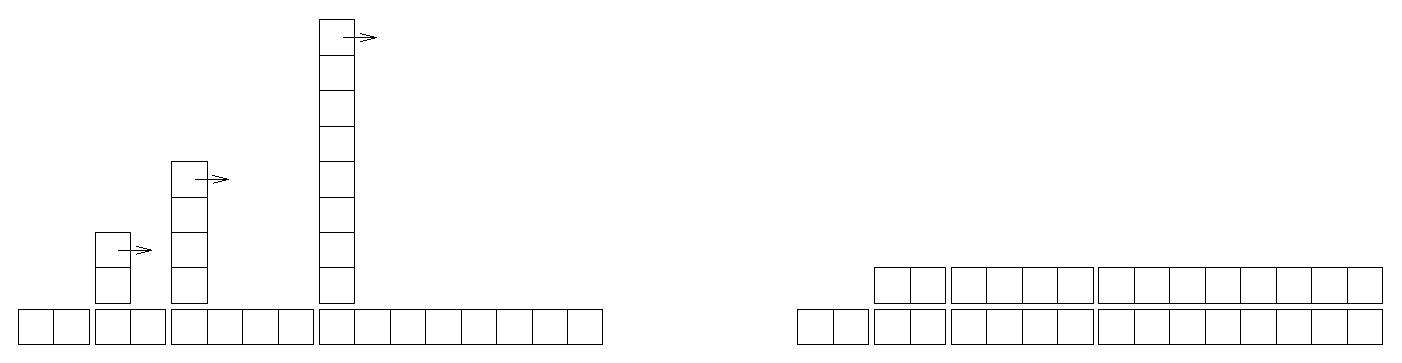
\includegraphics[width=3.0in]{figs/towers}}
\caption{Histogram of wealth with no tax.\label{fig.notax}}
\end{figure}

To compare the effect of taxation on wealth distribution, we need a
metric that measures how distributed or flat a certain wealth
distribution is.  We use the Gini coefficient, which is often used in
economics to measure the wealth gap (see
\url{http://en.wikipedia.org/wiki/Gini_coefficient}). The Gini
coefficient is between 0 and 1, with 0 the measurement of a perfectly
uniform distribution, and 1 the measurement of a distribution with
complete inequality.

Figure~\ref{fig.notax} shows a histogram describing the wealth
distribution when there is no tax system in place. For most initial
conditions without taxation, the Sugarscape quickly develops a
long-tailed distribution of wealth, skewed to the right. In these
cases, some agents die quickly, particularly in an environment with
many agents or one with low sugar regrowth rate. The separation
between the rich and the poor is significant, and there aren't many
agents occupying the middle ground. This is seen in real life in
societies where there is no tax structure and there isn't much of a
middle class.


\section{Reductionism or Holism?}

\begin{figure}[ht]
\centerline{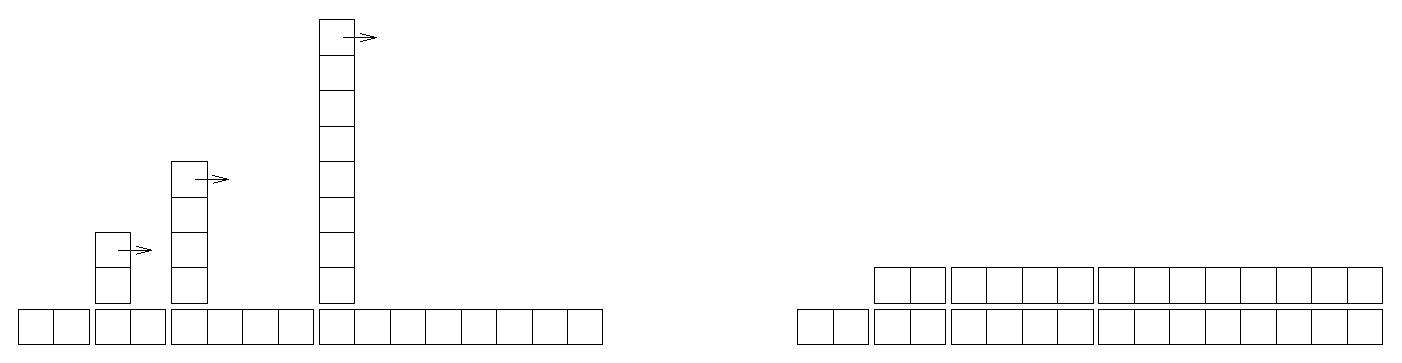
\includegraphics[width=3.0in]{figs/towers}}
\caption{Histogram of wealth, with tax.\label{fig.withtax}}
\end{figure}

\begin{figure}[ht]
\centerline{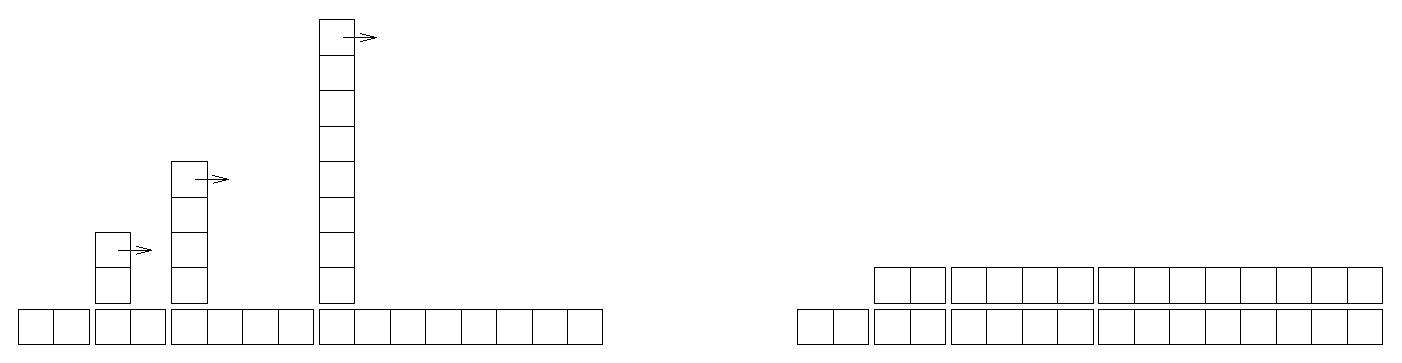
\includegraphics[width=3.0in]{figs/towers}}
\caption{The Gini coefficient versus the tax rate.\label{fig.gini}}
\end{figure}

Figure~\ref{fig.withtax} shows the effect of a relatively high tax
rate. The agents have a similar amount of sugar, and the economy has a
low Gini coefficient, 0.02.

Figure~\ref{fig.gini} shows that
higher taxes in general result in lower Gini coefficients. This makes
sense, since the point of our tax system is to redistribute
wealth.

\begin{figure}[ht]
\centerline{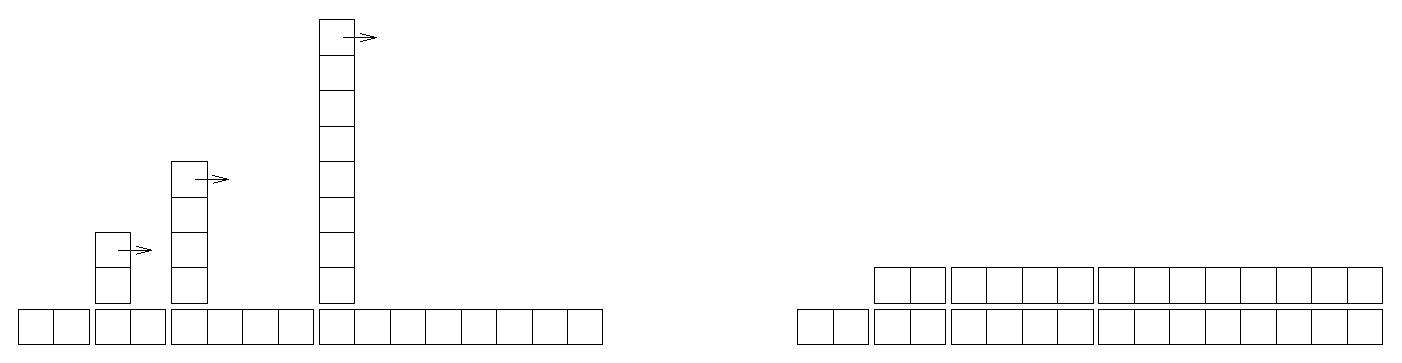
\includegraphics[width=3.0in]{figs/towers}}
\caption{Mean wealth versus tax rate.\label{fig.wealth}}
\end{figure}

In this model, perfect equality comes at a price.  With no taxation
the mean wealth was 358; with a 20\% tax rate it drops to 157.
Figure~\ref{fig.wealth} shows the effect of tax rate on wealth;
mean wealth gets smaller as taxes get higher.



\section{Instrumentalism and Music}

\begin{figure}[ht]
\centering{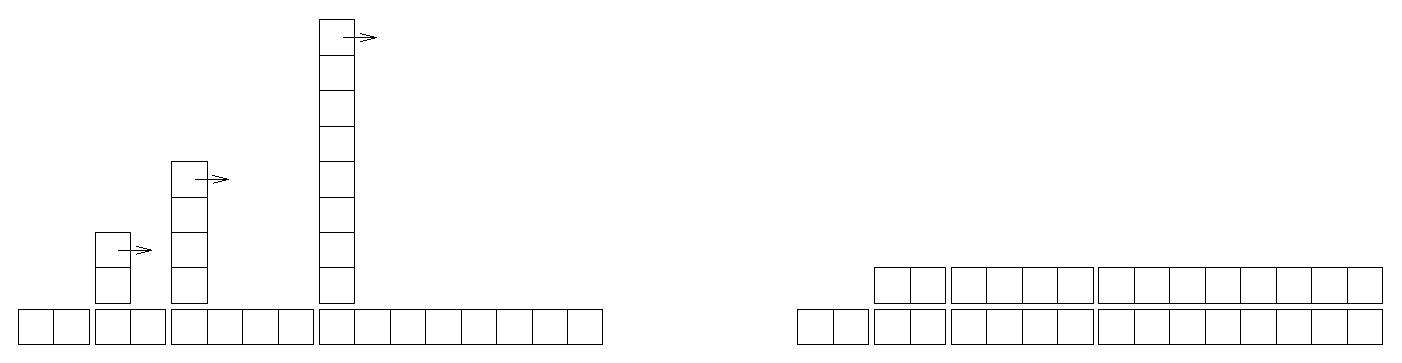
\includegraphics[width=3.0in]{figs/towers}}
\caption{Bottom quartile value versus tax rate. At 4\% the average wealth of the bottom quartile is maximized.\label{fig.optimal}}
\end{figure}

%\begin{figure}[ht]
%\centerline{\includegraphics[width=3.0in]{figs/pmf_2percent.pdf}}
%\caption{The wealth distribution for a smaller tax rate (2\%). There is still s%ome deviation, but the mean wealth is high.}
%\end{figure}

It's up to a society to determine its ideal wealth distribution. 
In our model, there is a conflict between the goals of maximizing
total wealth and minimizing inequality.

One way to reconcile this conflict is to maximize the wealth of
the bottom quartile.  Figure~\ref{fig.optimal} shows the mean
wealth of the poorest 25\% for a range of tax rates.  The optimal
tax rate is around 4\%.  At lower rates, there is more total
wealth, but the poor do not share it.  At higher rates, the poor
have a bigger share of a smaller pie.

Of course, this result depends on the details of our Sugarscape,
especially the model of productivity.  But this simple model
provides a way to explore relationships between wealth creation,
taxation and inequality.

\begin{exercise}

You can download our implementation of Sugarscape from
\url{thinkcomplex.com/Sugarscape.zip}.  Launch it by running
{\tt Gui.py}.  The sliders allow you to control the parameters
of the simulation.  Experiment with these parameters to see what
effect they have on the distribution of wealth.

\end{exercise}

\begin{exercise}

You can download our implementation of Sugarscape from
\url{thinkcomplex.com/Sugarscape.zip}.  Launch it by running
{\tt Gui.py}.  The sliders allow you to control the parameters
of the simulation.  Experiment with these parameters to see what
effect they have on the distribution of wealth.

\end{exercise}

\end{document}
